\documentclass[12pt, letterpaper]{article}
\usepackage[utf8]{inputenc}
\usepackage[russian]{babel}
\usepackage{amsmath}
\usepackage{xfrac}
\usepackage[document]{ragged2e}

\title{Устный Зачёт по Геометрии}
\author{Скорбенко Егор}
\date{Апрель 2018}

\begin{document}
\maketitle
\tableofcontents

\section {Дайте определение угла между векторами, скалярного произведения векторов. Сформулируйте условие перпендикулярности. Докажите теорему о вычислении скалярного произведения векторов через их координаты. Выведите формулу для вычисления угла между векторами.}
\subsection{Определения}
Угол между векторами- угол между направлениями этих векторов.\\
Скалярным произведением двух векторов называется произведение их длин на косинус угла между ними. \\
Условие перпендикулярности- скалярное произведенеие ненулевых векторов равно нулю тогда и только тогда, когда эти векторы перпендикулярны. \\
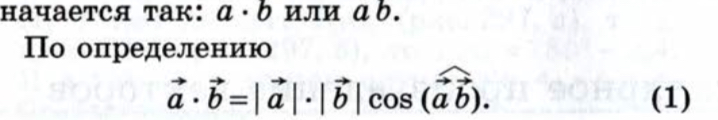
\includegraphics[scale=0.3]{photo.jpg} \\
\subsection {Теорема о вычислении скалярного произведения векторов через их координаты.}
В прямоугольной системе координат скалярное произведение векторов $\vec{a}$ и $\vec{b}$ выражается формулой \\
\begin{center}
$\vec{a}*\vec{b}={x_1}{x_2}+{y_1}{y_2}$
\end{center}
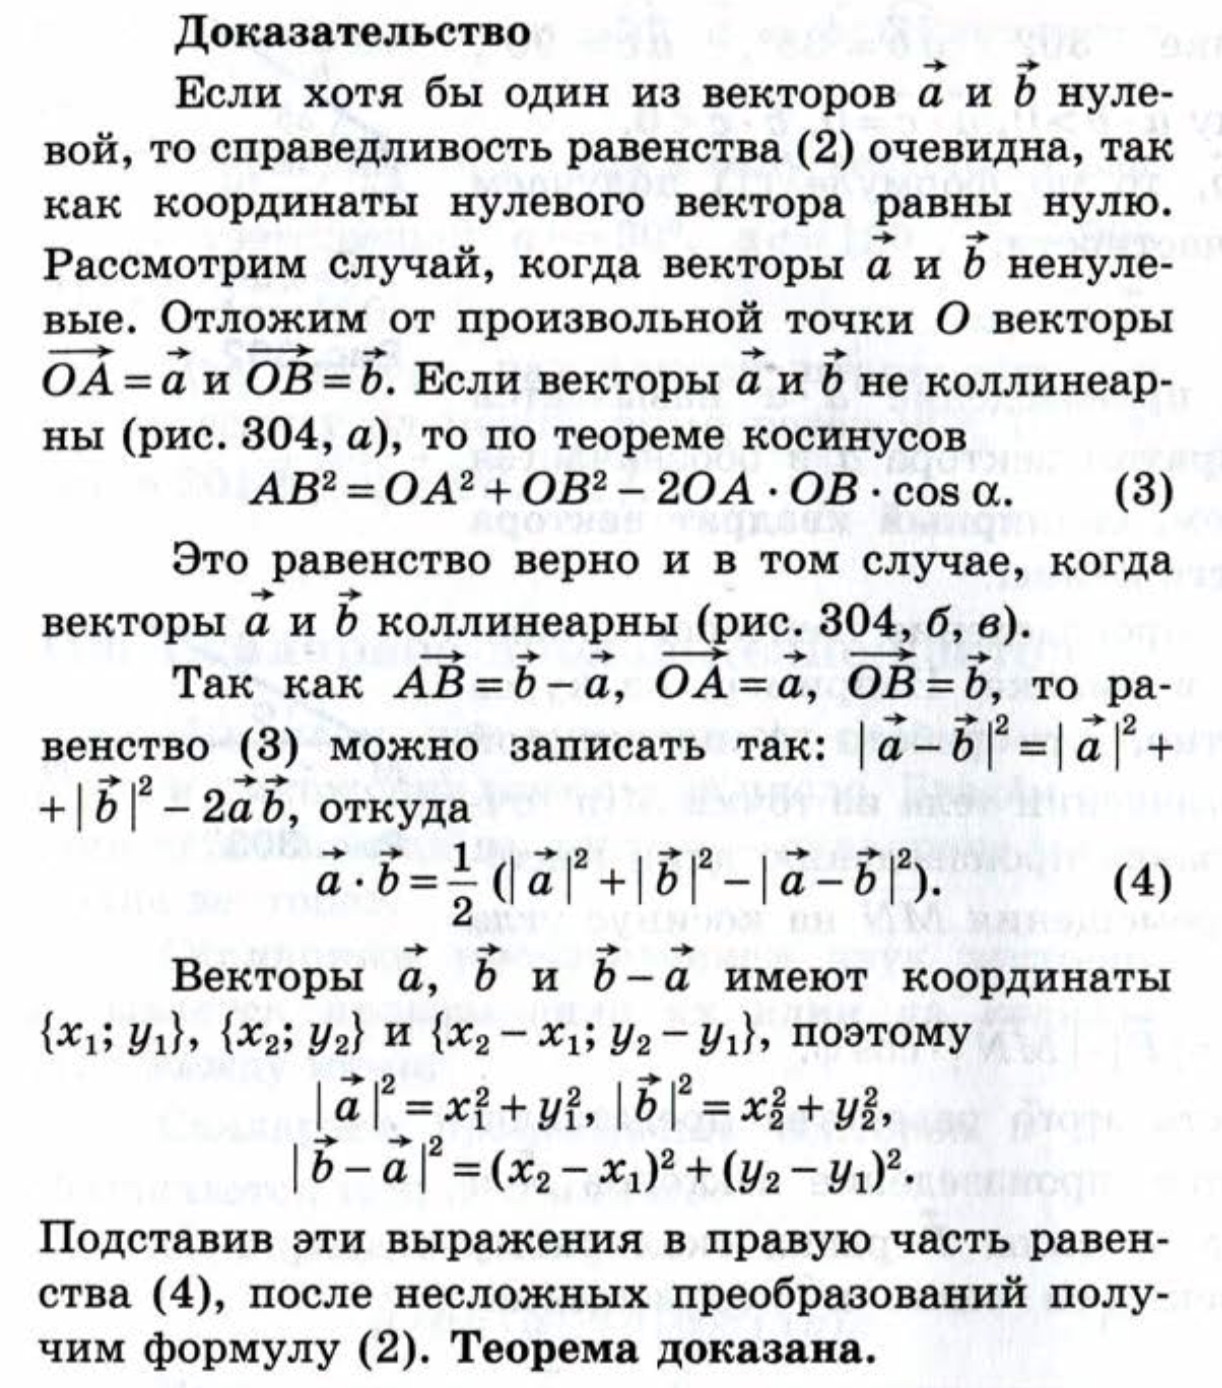
\includegraphics[scale=0.3]{photo2.jpg} \\
\subsection {Вывод формулы для вычисления угла между векторами.}
Углом между двумя векторами, отложенными от одной точки, называется кратчайший угол, на который нужно повернуть один из векторов вокруг своего начала до положения сонаправленности с другим вектором. \\
Косинус угла между векторами равен скалярному произведению векторов, деленному на произведение модулей векторов. \\
\begin{center}
$ \cos a =\dfrac{\overline{a}*\overline{b}}{\dfrac{}{\left|a\right|}*{\left|b\right|}} $
\end{center}


\section {Сформулируйте и докажите свойства скалярного произведения векторов.}
108

\section {Дайте определение правильного многоугольника. Докажите, что около любого правильного многоугольника можно описать окружность.}
109-110

\section {Дайте определение правшгьного многоугольника. докажите. по в любой правильный многоугольник можно вписать окружность.}
109, 111

\section {Выведите формулы для вычисления элементов правильного многоугольника (длина стороны, радиус вписанной окружности,  площадь) через радиус описанной окружности.}
112

\section {Выведите формулы для вычисления элементов правильного многоугольника (радиус описанной окружности, радиус вписанной окружности, площадь) через длину стороны.}

\section {Выведите формулы для вычисления радиуса описанной окружности и радиуса вписанной окружности в произвольном треугольнике}
114

\section {Дайте определения градуса и радиана. Выразите приближенное значение одного радиаиа в градусах. Выведите формулы для нахождения длины дуги через ее градусную меру и радианную.}
115 116

\section {Выведите формулы для нахождения площадей частей крута. }

\section {Сформулируйте свойства и признаки равнобедренной трапеции. Сформулируйте и допишите свойство равнобедренной трапеции с перпендикулярными диагоналями.}
\section {Дайте определение движения. сформулируйте общие свойства. Перечислите виды движений и их свойства.}
117-118
\section {Докажите теорему о произведении отрезков пересекающихся хорд окружности. докажите теорему о произведении отрезков секущей и квадрате касательной, проведенных из одной точки.}
пункт 73 последняя теорема + телеграм фото

\section {Сформулируйте и докажите теорему о величине угла между касательной и хордой.}
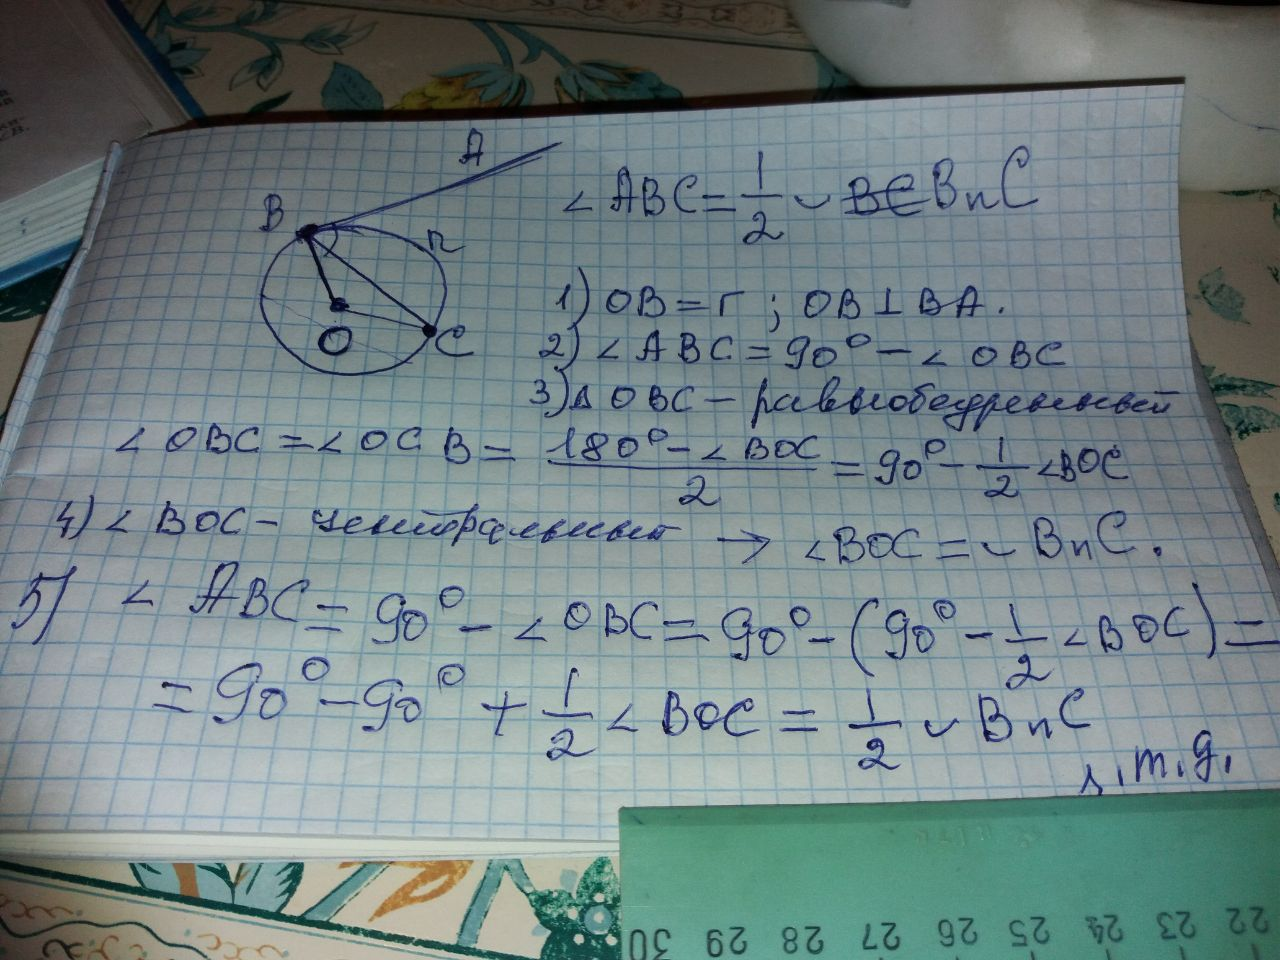
\includegraphics[scale=0.3]{asset-2.png} \\

\section {Сформулируйте и докажите теоремы о величине углов между пересекающимися хордами, между секущими.}
\includegraphics[scale=0.3]{asset-3.jpg} \\
\textbf{задача 661 + notability доказано, вставить картинкой} \\

\section {Сформулируйте и докажите теорему о сумме квадратов диагоналей параллелограмма.}
в предыдущем зачете

\section {Сформулируйте и докажите свойство диагоналей параллелограмма и формулу для вычисления длины медианы.}
в предыдущем зачете

\section {Сформулируйте признаки подобия треугольников. Докажите один из них по выбору.}
выучить сам- 61-63 пункт, 59 для определений

\section {Сформулируйте и докажите обобщенную теорему синусов.}
в предыдущем зачете

\section {Выведите формулы для нахождения пропорциональных отрезков в прямоугольном треугольнике. Выведите формулу для нахождения высоты прямоугольного треугольника через его стороны.}
в предыдущем зачете

\section {Выведите формулы для нахождения площади треугольника. (Не менее 4)}
\subsection {Стандартная}
$S=\dfrac{1}{2}ah $ \\
\textbf{Доказательство:} достроим до параллелограмма ABCD,\\
$\Delta ABC = \Delta DCB = \dfrac{1}{2}ABCD. $ \\

\subsection {Формула Герона}
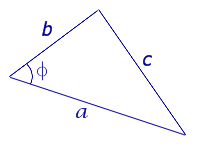
\includegraphics[scale=1]{asset.png} \\
$S=sqrt(p(p-a)(p-b)(p-c))$ \\
$p=\dfrac{P}{2}=\dfrac{a+b+c}{2}$ \\
\textbf{Доказательство:} \\
\begin{flushleft}
$S=\dfrac{1}{2}absin\phi$ => $S^2=\dfrac{1}{4}a^2b^2sin^2\phi=\dfrac{1}{4}a^2b^2(1-cos^2\phi).$ \\
$c^2=a^2+b^2-2abcos\phi$ => $cos\phi=\dfrac{a^2b^2-c^2}{2ab}=cos^2\phi$\\
$S^2=\dfrac{1}{4}a^2b^2(1-cos^2\phi)= $ \\
$ \dfrac{1}{4}a^2b^2(1-(\dfrac{a^2+b^2-c^2}{2ab})^2)=$ \\
$ \dfrac{1}{16}(4a^2b^2-(a^2+b^2-c^2)^2)= $ \\
$ \dfrac{1}{16}((a+b)^2-c^2)(c^2-(a-b)^2)= $ \\
$ \dfrac{1}{16}(a+b+c)(a+b-c)(c+a-b)(c-a+b)= $ \\
$ \dfrac{1}{16}(a+b+c)(a+b+c-2c)(c+a+b-2b)(a+b+c-2a)= $ \\ 
$ \dfrac{1}{16}2p(2p-2c)(2p-2b)(2p-2a)= p(p-c)(p-b)(p-a)$ \\
\end{flushleft}
\textbf{$S=sqrt(p(p-a)(p-b)(p-c))$ ЧТД.}

\subsection {Полупериметр и вписанная окружность}
$S=\dfrac{1}{2}Pr$ \\

\subsection{Формула через синус}
$S=\dfrac{1}{2}ab*sin\alpha $ \\

\section {Выведите формулу площади произвольного четырехугольника и формулу площади дельтоида.}
\section {Сформулируйте и докажите теорему о центре окружности, вписанной в треугольник. Сформулируйте и докажите теорему о центре окружности, описанной около треугольника.}
\section {Сформулируйте и докажите свойство биссектрисы треугольника.}
\section {Сформулируйте и докажите свойство биссектрис параллелограмма.}
\section {Сформулируйте и докажите три свойства равнобедренной трапеции}
\section {Сформулируйте и докажите признаки прямоугольного треугольника. (Теорема, обратная теореме Пифагора и соотношение медианы и стороны, к которой она приведена.}
\section {Выведите формулы для нахождения радиусов вписанной и описанной окружностей через стороны правильных треугольника, квадрата и шестиугольника.}
\section {Дайте определение вписанного угла. Сформулируйте и докажите теорему о величине вписанного угла.}
\section {Сформулируйте и докажите свойство медиан в произвольном треугольнике.}
\section {Сформулируйте теорему Чевы. Сформулируйте и докажите теорему Менелая.}
\section {Сформулируйте и докажите свойства площадей треугольников с равными высотами, треугольников с равным углом и треугольников справными основаниями.}
\section {Сформулируйте и докажите свойства вписанного и описанного четырехугольника.}
\section {Найдите радиус вписанной и описанной окружностей прямоугольного треугольника.}
\section {Сформулируйте и докажите условия перпендикулярности и коллинеарность векторов через их координаты.} 

\end{document}